%Start
%required packages and reason
\documentclass[11pt]{article}
\usepackage[a4paper,margin=1in]{geometry}
\usepackage{mathtools} % required for sigma notation
\usepackage{graphicx} %required to load images
\usepackage{amsmath} %required for the matrices
\usepackage{upgreek} %required for Greek symbols
\usepackage{xfrac} %for differentiation symbol
\usepackage{float} %to set the figures exactly where we want,(\figure "[H]")
\usepackage{listings} %to get colorful code in latex
\usepackage{color} %to get a nice color scheme
\usepackage{pythonhighlight} %to make the the python codes nice

%initial headings
\title{EE2703 Assignment 5: The Resistor Problem}
\author{Anvith Pabba EE19B070}
\date{25th March 2021}

%begin document
\begin{document}

\maketitle

\section{Introduction}
In this assignment, we wish to find the currents and voltages produced in the given resistor. In order to obtain these values, we use suitable approximations. We then visualize the data in the form of various plots. 

\section{The Resistor Problem}
\subsection{Given info}
In the given question, A wire is soldered to the middle of a copper plate and its voltage is held at 1 Volt. One side of the plate is grounded, while the remaining are kept floating. The plate is Ny cm x Nx cm in dimensions.

\subsection{The Given Figure}
\begin{figure}[H]
    \centering
    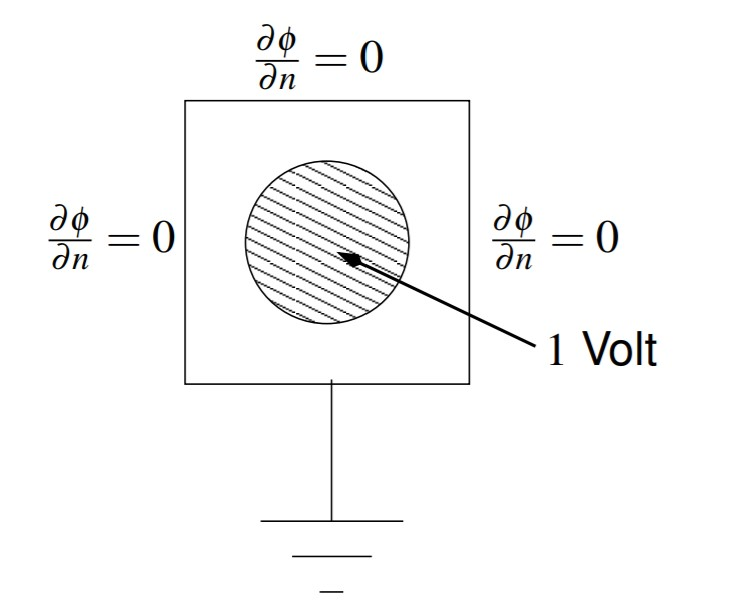
\includegraphics[scale = 1]{Problem_1.jpg}
    \caption{Visual representation of the problem}
\end{figure}

\section{Theory}

\subsection{Solving the equations}
The conductivity is given by:
\begin{equation}
    \Vec{\textit{j}}= \sigma\Vec{\textit{E}}
\end{equation}
Now the Electric field is the gradient of the potential:
\begin{equation}
    \Vec{\textit{E}}= -\nabla\phi
\end{equation}
and continuity of charges yields:
\begin{equation}
    \nabla.\Vec{\textit{j}}=- \frac{\partial \rho}{\partial t} 
\end{equation}
Combining these two equations and assuming the conductivity of the medium is constant and is $\sigma$ gives us:
\begin{equation}
    \nabla^2\phi= \frac{1}{\sigma} \frac{\partial \rho}{\partial t} 
\end{equation}
For DC currents, the RHS is zero, this gives us:
\begin{equation}
    \nabla^2\phi= 0
\end{equation}

\subsection{Approximations to solve in 2-D}
Laplace’s equation is easily transformed into a difference equation. The equation can be written out in Cartesian coordinates:
\begin{equation}
    \frac{\partial^2 \phi}{\partial x^2} + \frac{\partial^2 \phi}{\partial y^2} = 0
\end{equation}
assuming $\phi$ is available at points $(x_j,y_j)$, we can write:
\begin{equation}
    \frac{\partial \phi}{\partial x} \Biggr|_{(x_j,y_j)}^{} = \frac{\phi(x_j_+_1_/_2,y_j) - \phi(x_j_-_1_/_2,y_j)}{\Delta x}
\end{equation}
and
\begin{equation}
    \frac{\partial^2 \phi}{\partial x^2} \Biggr|_{(x_j,y_j)}^{} = \frac{\phi(x_j_+_1,y_j) - 2\phi(x_j,y_j) + \phi(x_j_-_1,y_j)}{(\Delta x)^2}
\end{equation}
Combining this with the corresponding equations for the y-derivatives, we finally get:
\begin{equation}
    \phi_i_,_j = \frac{\phi(x_j_+_1,y_j) +\phi(x_j_-_1,y_j) +\phi(x_j,y_j_+_1) +\phi(x_j,y_j_-_1) }{4}
\end{equation}

Thus, if the above solution holds, the potential at any point should be the average of its neighbours.

\subsection{Boundary Conditions}
At boundaries where the electrode is present, just put the value of
potential itself. At boundaries where there is no electrode, the current should be tangential because charge can’t leap out of the material into air. Since current is proportional to the Electric Field, what this means is the gradient of $\phi$ should be tangential. This is implemented by requiring that $\phi$ should not vary in the normal direction.

\section*{Writing The Code}
\setcounter{section}{0} %sets the section counter back to 0
\section{Getting the parameters}
\subsection{Getting the initial parameters}
We have 4 initial parameters, \textbf{Nx, Ny, Radius, Niter}. We get these 4 parameters from the user. We get these parameters through the user:

\begin{figure}[H]
    \centering
    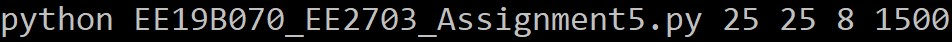
\includegraphics[scale = 1.25]{Pic_1.jpg}
    \caption{How the code should be executed}
\end{figure}

After extracting the inputs through \textit{import sys}, we check if everything is correct or if there are any mistakes from the users side.
We check the following:

\begin{enumerate}
    \item All 4 parameters \textbf{must be given}
    \item \textit{Nx, Ny, Radius, Niter} should \textbf{all be integers}
\end{enumerate}

We check whether the conditions above are satisfied, if they are not then an error is given to the user. The relevant code:

\begin{python}
import sys

#Checking if correct number of arguments are given
if len(sys.argv)!=5:
	print("Please enter ALL 4 parameters!!")

#Checking if all the inputs are intgers
while True:
	try:
		Nx = int(sys.argv[1])       
	except ValueError:
		print('argument 1 must be an integer')
		break
	else:
		Nx = int(sys.argv[1])
		break 
		
\textbf{Similarly we do this for Nx,Ny,Radius and Niter}
\end{python}

\subsection{Initialising the phi (potential) and other arrays}
phi is a matrix of size Nx,Ny. It is initialed with initial value of 0.
\textbf{x} is the shifted x axis, such that the middle value is 0
\textbf{y} is the shifted y axis, such that the middle value is 0
X,Y is the corresponding meshgrid
we also define \textbf{n} and initialise \textbf{errors}

\begin{python}
x = np.linspace(-((Nx-1)/2), ((Nx-1)/2), Nx)
y = np.linspace(-((Ny-1)/2), ((Ny-1)/2), Ny) 

#initialising phi
phi = np.zeros([Ny,Nx])
X,Y=meshgrid(x,y)
n = arange(Niter)
errors = np.zeros([Niter,1])
\end{python}

\subsection{finding and initialising points with V = 1.0}
we use the \textbf{where} command to find points that satisfy the condition of $X*X +Y*Y <= (radius * radius)$, we store these points in an array \textit{ii}. We then make every point in this have a potential of V = 1 (given in the problem statement).

\begin{python}
ii = where((X*X + Y*Y) <= r*r)
phi[ii] = 1.0
\end{python}

\subsection{Plot of phi}
\begin{figure}[H]
    \centering
    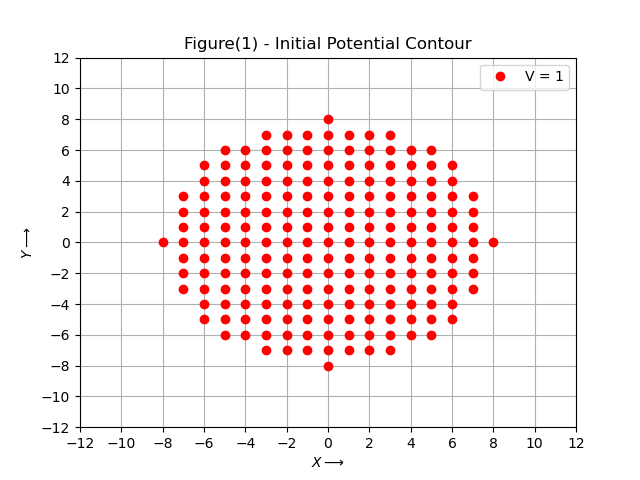
\includegraphics[scale = 1]{Figure_1.png}
    \caption{Initial plot of phi}
\end{figure}

\section{Performing the iterations}
\subsection{The iteration}
Using the theory given above, we know that the potential of each point is the average of the values around it. To get the required values of phi, we perform an iteration that comprises of 3 main parts:
\begin{itemize}
    \item [$\ast$] for k in range(Niter)
    \begin{enumerate}
        \item  save copy of phi
        \item  update phi array
        \item  assert boundaries
    \end{enumerate}
    \item [$\ast$] errors[k]=(abs(phi-oldphi)).max()
\end{itemize}

\subsection{Save copy of phi}
To do this, we use the \textbf{.copy()} command
\begin{python}
oldphi=phi.copy()
\end{python}

\subsection{updating the potential}
In order to perform the averaging function on every point in the phi array, we would have used 2 nested for loops. In reality, for loops are not as optimised in python as compared to vector loops, this means the time taken by the nested for loops is extremely high. Infact, for every nested for loop thats added, the time taken by the program increases exponentially. This is not at all favourable.

So instead of using for loops, we use vectorized code that performs the same functions. This vectorized code significantly reduces the time taken by the program.

so a conventional code:
\begin{python}
for(i=1 ; i<Ny-1 ; i++ ){ // interior nodes
    for(j=1 ; j<Nx-1 ; j++ ){ // interior nodes
        phinew[i,j]=0.25*(phi[i,j-1]+phi[i,j+1]+phi[i-1,j]+phi[i+1,j]);
        }
}
\end{python}

Is now converted to vectorized form, as:

\begin{python}
phi[1:-1,1:-1] = 0.25*(phi[1:-1,:-2] + phi[1:-1,2:] + phi[:-2,1:-1] + phi[2:,1:-1])
\end{python}

\subsection{Boundary conditions}
The theory for this is already given above, in the first Section 3.3.

At the \textbf{left boundary}, we need to set the normal derivative of 
potential to zero. This means that 

\begin{equation}
\frac{\partial \phi}{\partial x} = 0.
\end{equation}

We similarly do this for the \textbf{right side} and the \textbf{top side}.
Also, the voltage of the bottom is constant at 0, but this is automatically 
taken care of.

The voltages of the points in the wire might get overwritten, so we have to 
keep updating them after each iteration. We do this by using phi[ii] = 1.0.

\subsection{Code}
All the above in vectorized code is:
\begin{python}
    #assert boundaries
	phi[1:-1,0] = phi[1:-1,1]	#left side
	phi[1:-1,-1] = phi[1:-1,-2]	#right side
	phi[0,1:-1] = phi[1,1:-1]	#top side
	#bottom is fixed with a value of 0

	phi[ii] = 1.0
\end{python}

\section{Obtaining and Plotting the Errors}
Plotting the Errors in semilogy and loglog form

\begin{python}
title("Figure(2) - Error plot 1")
semilogy(n,errors,label="semilogy plot of error vs iteration")
xlabel('$n\longrightarrow$')
ylabel('$error,log[n]\longrightarrow$')
grid(True)
legend()
show()

title("Figure(3) - Error plot 2")
loglog(n,errors,label="loglog plot of error vs iteration")
xlabel('$n,log\longrightarrow$')
ylabel('$error[n],log\longrightarrow$')
grid(True)
legend()
show()
\end{python}

\subsection{Semilogy Plot}
\begin{figure}[H]
    \centering
    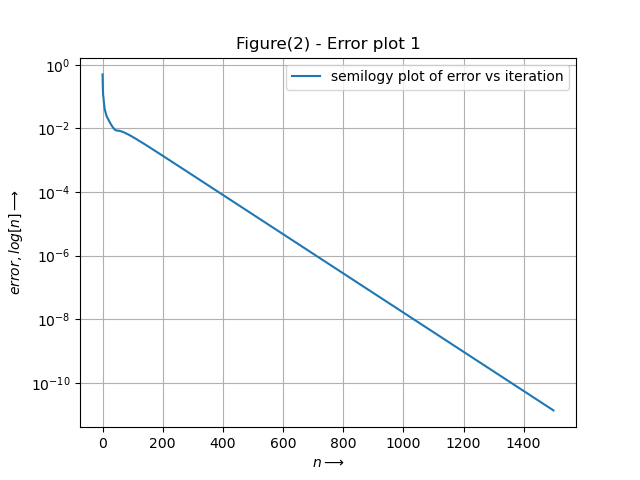
\includegraphics[scale = 1]{Figure_2.png}
    \caption{Semilogy plot of the error}
\end{figure}

\subsection{Loglog Plot}
\begin{figure}[H]
    \centering
    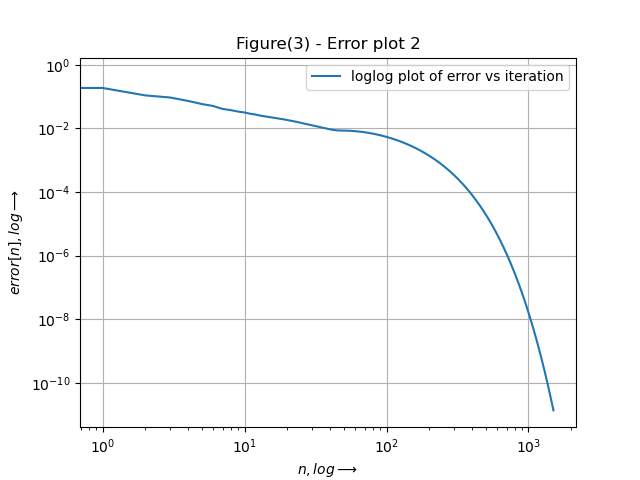
\includegraphics[scale = 1]{Figure_3.png}
    \caption{loglog plot of the error}
\end{figure}

\subsection{Semilogy Plot for errors after the 500th iteration}

As we can see from the first semilogy plot, there is a small deviation for the iterations less than 500. But for iterations greater than 500, the plot is a straight line. In order to test this, we plot the semilogy plot for iterations greater than 500.

\begin{figure}[H]
    \centering
    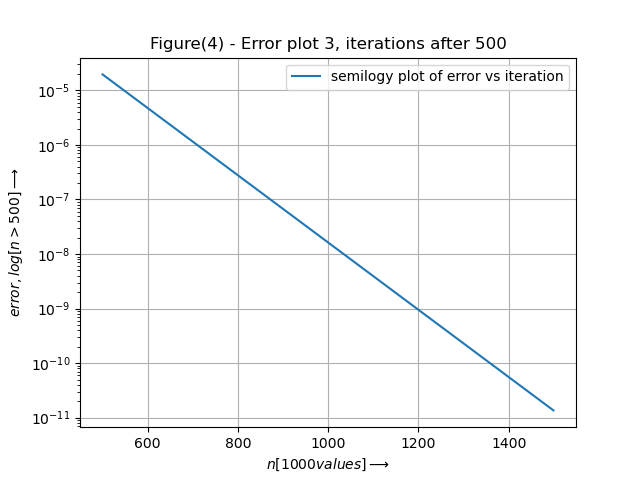
\includegraphics[scale = 1]{Figure_4.png}
    \caption{Semilogy plot of the error, for iterations $>$500}
\end{figure}

\subsection{Finding the Best fit for the errors}
As we can see form the graphs, the semilogy plot is a straight line this means that the error is of the form of:
\begin{equation}
    errors_k = Ae^{Bk}
\end{equation}

To obtain the best fit for A and B, we use lstsq on the linear equation obtained by taking the log of both sides. i,e:
\begin{equation}
    log(error_k) = log(A) + Bk
\end{equation}

We can see that taking the error as $Ae^{Bk}$ is not very correct for iterations less than 500. So, we find A and b for 2 different conditions.
1) for all iterations
2) only for iterations >500

\subsection{Code}
\begin{python}
fit1 = zeros([1000,1])
fit2 = zeros([1500,1])
#using lstsq
#lstsq for after 500
c1 = np.linalg.lstsq(c_[ones([1000,1]),n[500:1500]], log(errors[500:1500]),rcond = None)[0]
logA1 = c1[0]
A1 = exp(logA1)
B1 = c1[1]

#lstsq for the entire thing
c2 = np.linalg.lstsq(c_[ones([1500,1]),n], log(errors),rcond = None)[0]
logA2 = c2[0]
A2 = exp(logA2)
B2 = c2[1]
\end{python}

\subsection{Values obtained from lstsq method}
fitted values of A1 and B1 for iterations $>500$ are : 
\begin{itemize}
    \item A1 = [0.02378819] and
    \item B1 = [-0.01419784]
\end{itemize}

fitted values of A2 and B2 for all iterations are : 
\begin{itemize}
    \item A2 = [0.02370508] and
    \item B2 = [-0.0141953]
\end{itemize}
We can see that both obtained values of A and B are very similar.

\subsection{Semilogy Plot of obtained and actual errors}
We can see that all 3 semilogy plots are all the same.
\begin{figure}[H]
    \centering
    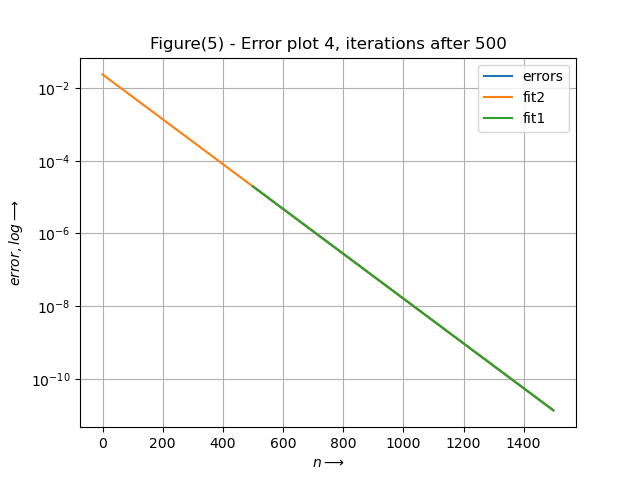
\includegraphics[scale = 1]{Figure_5.png}
    \caption{Semilogy plot of obtained and actual errors}
\end{figure}

\subsection{Loglog Plot of obtained and actual errors}
We can see that all 3 semilogy plots are all similar, but the actual error deviates for iterations $<500$.
\begin{figure}[H]
    \centering
    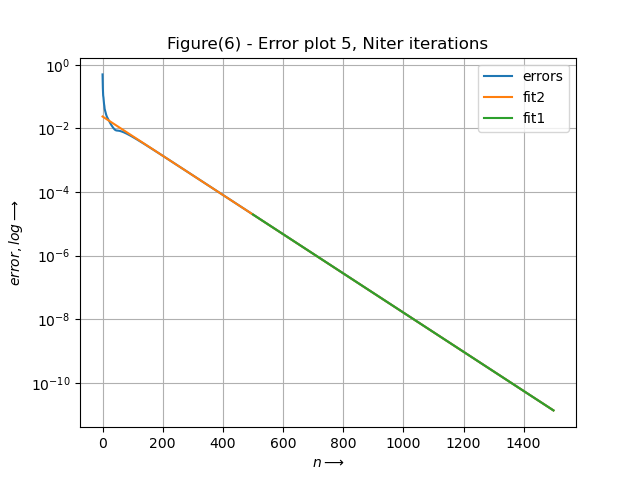
\includegraphics[scale = 1]{Figure_6.png}
    \caption{Loglog plot of obtained and actual errors}
\end{figure}

\subsection{Stopping Error}
The approximate Error obtained is:
\begin{equation}
    Error \approx -\frac{A}{B}e^{B(N + 0.5)}
\end{equation}
Error we obtain is:
\begin{equation}
    Error = \frac{0.02370508}{-0.0141953} e^{-0.0141953*1500}
\end{equation}
this is equal to:   1.6699*5.67*1e-10 \\
which is \textbf{9.4466*1e-10}

\section{Contour plot of potential}
This plots the voltages as contours with colorbar variations.

\subsection{Code}
\begin{python}
title("Figure(9) - The contour plot")
contourf(x, -y, phi)
colorbar()
plot(ii[0] - (Nx-1)/2, ii[1] - (Ny-1)/2,linestyle="None", color='red', marker='o',label="V = 1")
xlabel("$x\longrightarrow$")
ylabel("$y\longrightarrow$")
show()
\end{python}

\subsection{Plot}
\begin{figure}[H]
    \centering
    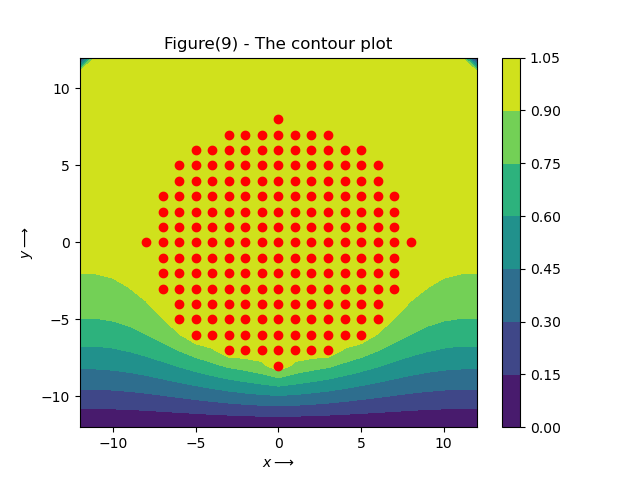
\includegraphics[scale = 1]{Figure_10.png}
    \caption{Contour plot}
\end{figure}

\section{3-D Surface plot}
we use the \textit{mpl$_$toolkits.mplot3d.axes3d} with alias \textit{p3} command to plot.

\subsection{Code}
\begin{python}
title("Figure(8) - The 3-D surface plot of the potential")
fig1=figure(8) # open a new figure
ax=p3.Axes3D(fig1) # Axes3D is the means to do a surface plot
surf = ax.plot_surface(Y, X, phi.T, rstride=1, cstride=1, cmap=cm.jet)
ylabel('$Ground$')
xlabel('$y\longrightarrow$')
show()
\end{python}

\subsection{Plot, view 1}
\begin{figure}[H]
    \centering
    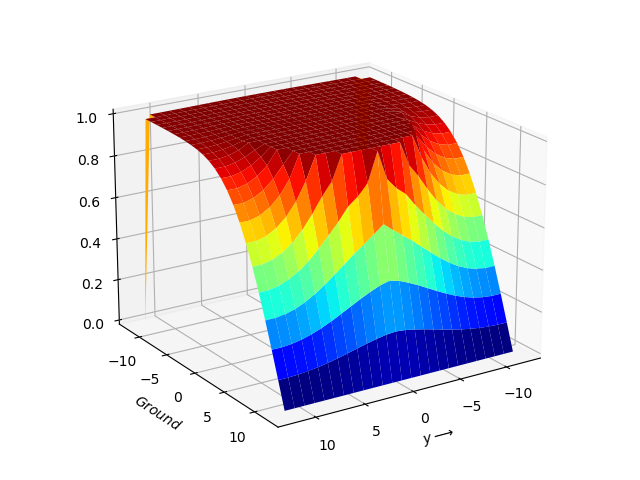
\includegraphics[scale = 1]{Figure_8.png}
    \caption{surface plot, view 1}
\end{figure}

\subsection{Plot, view 2}
\begin{figure}[H]
    \centering
    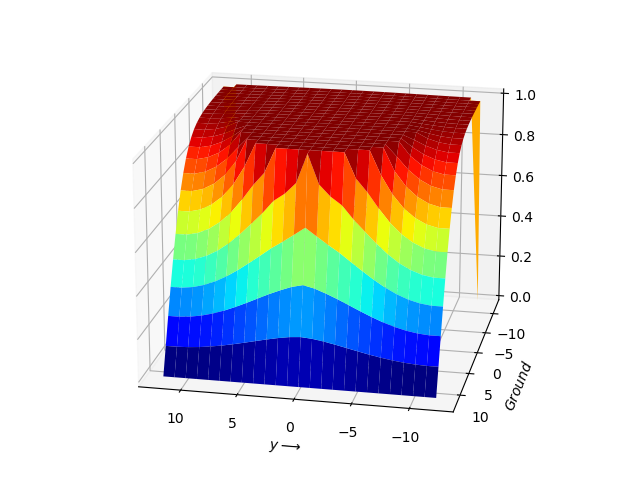
\includegraphics[scale = 1]{Figure_9.png}
    \caption{surface plot, view 2}
\end{figure}

\section{Quiver Plot of The Currents}

Now to obtain the currents, we need to compute the gradient. Our equations are:
\begin{equation}
    j_x = -\frac{\partial \phi}{\partial x}
\end{equation}
\begin{equation}
    j_y = -\frac{\partial \phi}{\partial y}
\end{equation}
\textbf{The actual value of $\sigma$ does not matter to the shape of the current profile, so we set it to unity.}\\
This numerically translates to:
\begin{equation}
    J_x_,_i_,_j = \frac{1}{2}(\phi_i_,_j_-_1 - \phi_i_,_j_+_1)
\end{equation}
\begin{equation}
    J_y_,_i_,_j = \frac{1}{2}(\phi_i_-_1_,_j - \phi_i_+_1_,_j)
\end{equation}

\subsection{Code for Currents}
This is the vectorized form of the code
\begin{python}
Jx = np.zeros([Ny,Nx])
Jy = np.zeros([Ny,Nx])

#Jx,Jy for the quiver

Jx[1:-1, 1:-1] = 0.5*(phi[1:-1, 0:-2] - phi[1:-1, 2:])
Jy[1:-1, 1:-1] = 0.5*(phi[2:, 1:-1] - phi[0:-2, 1:-1])
\end{python}

\subsection{Code to plot the quiver plot}
\begin{python}
title("Figure(7) - Current quiver plot")
quiver(x,y,Jx[::-1,:],Jy[::-1,:],scale = 5,label = "current")
plot(ii[0] - (Nx-1)/2, ii[1] - (Ny-1)/2,linestyle="None", color='red', marker='o',label="V = 1")
xlabel('$x\longrightarrow$')
ylabel('$y\longrightarrow$')
grid(True)
legend(loc = 'upper right')
show()
\end{python}

\subsection{Quiver plot}
\begin{figure}[H]
    \centering
    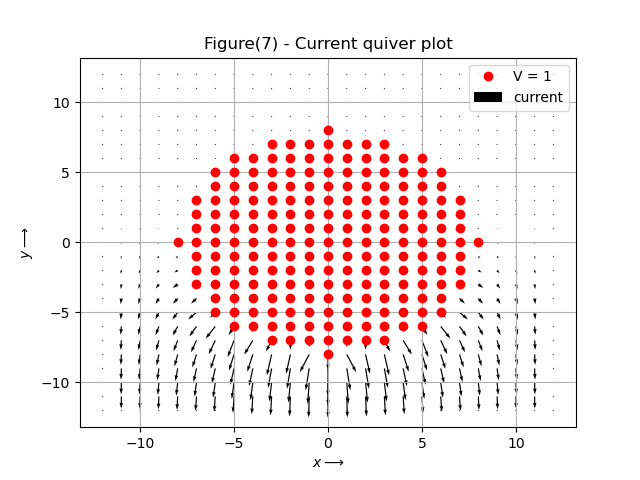
\includegraphics[scale = 1]{Figure_7.png}
    \caption{Quiver plot of the currents}
\end{figure}

\section{Observations}
\begin{enumerate}
    \item We can clearly see that most current flows in the bottom of the plate, from the wire to the grounded side. And that there is almost no current in the rest of the plate.
    \item we know from Ohms law, 
    \begin{equation}
         \Vec{\textit{j}}= \sigma\Vec{\textit{E}}
    \end{equation}
    and this tells us that the electric field is much higher in the lower part pf the plate as compared to the rest of the plate.
    \item As the current as well as the electric field is higher in these regions, the ohmic loss is very high and centralized. Hence the temperature in these areas is also going to be extremely high. When modelling such a device, we need to be very careful it can handle the high temperatures.
    \item in order to improve accuracy, we can increase Nx and Ny, but this will also increase the time the program takes. This is only required if we require higher accuracy over time.
\end{enumerate}

\section{Conclusions}
\begin{enumerate}
    \item In conclusion, we see that most current flows in the bottom of the plate, this will strongly heat it up and raise its temperature.
    \item We learnt how to plot data in the form of contours and 3d surface plots.
    \item we learnt how to plot the quiver plots, and how to find the current through vectorized code.
    \item We saw how to improve the run time of our program by using vectorized code instead of un-optimized \textit{for} loops.
    \item we saw that the error is very close to the exponential form of $Ae^{Bk$ and that the values obtained by lstsq method are also extremely similar.
\end{enumerate}























%end document
\end{document}
